\chapter{Metodologia}
\label{sec:Metodologia}

Neste capítulo serão apresentados os métodos, ferramentas e o processo definido
para aplicação no presente trabalho visando alcançar o seu objetivo final.

  As seções estão dispostas em:

  \begin{enumerate}
    \item \textbf{Levantamento bibliográfico} Define os métodos utilizados para
    a realização das pesquisas e levantamento bibliográfico.
    \item \textbf{Metodologia de pesquisa} Descrição do fluxo que será
    adotado para análise dos fatores pertinentes ao escopo do presente trabalho.
    \item \textbf{Metodologia de desenvolvimento} Descrição dos métodos
    aplicados a gestão do presente projeto, visando alcançar seu objetivo final.
    \item \textbf{Ferramentas} Breve descrição das tecnologias e ferramenas
    que serão utilizados.
  \end{enumerate}

\section{Levantamento bibliográfico}

Para referenciamento deste trabalho foram realizados estudos acerca de
\textit{startups}, desenvolvimento de software e aspectos relacionados
a escalabilidade de um sistema por meio de livros, Google Scholar, dentre
outras fontes. Os tópicos abordados dentro de cada tema foram selecionados
com base na sua respectiva importância dentro do assunto e no seu envolvimento
no contexto da Rua Dois. Individualmente, os temas citados são bem explorados e
abordados pela comunidade acadêmica, contudo, quando relacionados os artigos e
estudos a respeito tendem a ser mais escassos.

Publicações e palestras de empresas de referencia voltadas ao desenvolvimento de
software no contexto de \textit{startups} também foram utilizadas com o intuito de
contribuir com perspectivas mais atuais a respeito do tema.

\section{Metodologia de pesquisa}
\label{sec:MetodologiaPesquisa}

Pretende-se com este trabalho realizar um estudo de caso acerca do desenvolvimento
de software na empresa Rua Dois, considerando os aspectos que são pertinentes para
uma \textit{startup}. Para tal, será realizada uma comparação entre duas arquiteturas
de software distintas adotadas dentro da Rua Dois para um mesmo sistema. Ao final,
com os resultados obtidos desta comparação e com base em estudos realizados por meio
de pesquisa exploratória pretende-se elencar boas práticas e recomendações para o
desenvolvimento de software na empresa. Dessa forma, esta seção visa descrever
os objetos de análise, os aspectos a serem considerados na análise comparativa e
como se dará a análise final.

\subsection{Objetos de análise}

O desenvolvimento do sistema da Rua Dois foi marcado por duas fases distintas.
Estas fases serão abordadas na \autoref{sec:ArquiteturaDoSistema} e serão
os objetos de análise do presente trabalho para a realização da análise
comparativa. A seguir é apresentada uma breve descrição sobre cada fase:

    \begin{description}
        \item [Fase 1] Fase inicial de desenvolvimento do software da Rua Dois,
        marcado por uma arquitetura de microsserviços e constantes alterações
        no software visando validar ideias.
        \item [Fase 2] Segunda fase de desenvolvimento do software da Rua Dois,
        marcado por uma arquitetura monolítica e um escopo melhor definido.
    \end{description}

\subsection{Etapas do desenvolvimento}

O desenvolvimento do presente trabalho acontecerá nas seguintes etapas:

    \begin{description}
        \item[Etapa 1] Estudo acerca da arquitetura adotada em cada fase;
        \item[Etapa 2] Coleta e levantamento de dados pertinentes aos aspectos que serão
        considerados para realização da análise comparativa;
        \item[Etapa 3] Análise comparativa entre os dados coletados;
        \item[Etapa 4] Definição de diretrizes acerca do desenvolvimento de software
        escalável na Rua Dois.
    \end{description}

A seguir segue a descrição de cada etapa.

\subsubsection{Etapa 1: Estudo acerca das arquiteturas adotadas}

Pretende-se nesta etapa descrever os elementos arquiteturais adotados em cada fase,
quais tecnologias foram utilizadas, quais as dificuldades encontradas e o contexto
da empresa e suas respectivas fases.

\subsubsection{Etapa 2: Coleta e levantamento de dados}
\label{sec:Etapa2}

Para os objetos de análise definidos serão levantados os seguintes dados e informações
julgados como pertinentes para a análise final:

    \begin{description}
        \item [Qualidade de código] Usando métricas de qualidade de código pretende-se
        avaliar questões referentes a coesão e acoplamento do sistema em cada uma das
        fases.
        \item [Práticas de desenvolvimento de Software] Elencar quais práticas de
        desenvolvimento de software foram aplicadas em cada fase e como estas práticas
        afetaram a qualidade do sistema em questão.
        \item [Nível de conhecimento e experiência da equipe no contexto de \textit{startups}]
        Aplicação de um questionário entre os membros do time de desenvolvimento participantes
        de cada fase, com o intuito de avaliar o domínio do time com as tecnologias utilizadas
        e a experiência com desenvolvimento de software dentro de \textit{startups}.
        \item [Tecnologias utilizadas] Identificar quais foram as tecnologias utilizadas em
        cada fase, como elas influenciaram o desenvolvimento e qual a escalabilidade de cada
        tecnologia.
        \item [Escalabilidade do sistema] Por meio de testes de escalabilidade, coletar
        informações sobre o nível de escalabilidade da arquitetura adotada em cada fase.
        \item [Relação com o ciclo de vida de uma \textit{startup}] Avaliar qual foi o
        contexto de desenvolvimento com base nas fases de uma \textit{startup} e como a
        arquitetura adotada influenciou nesse contexto.
    \end{description}

Para cada um dos itens definidos será executado o processo ilustrado na
\autoref{fig:ProcessoAnaliseComparativa} com o propósito de definir os métodos utilizados
e coletar os dados.

    \begin{figure}[h]
      \caption{Processo para realização da coleta de dados\label{fig:ProcessoAnaliseComparativa}}
      \centering
      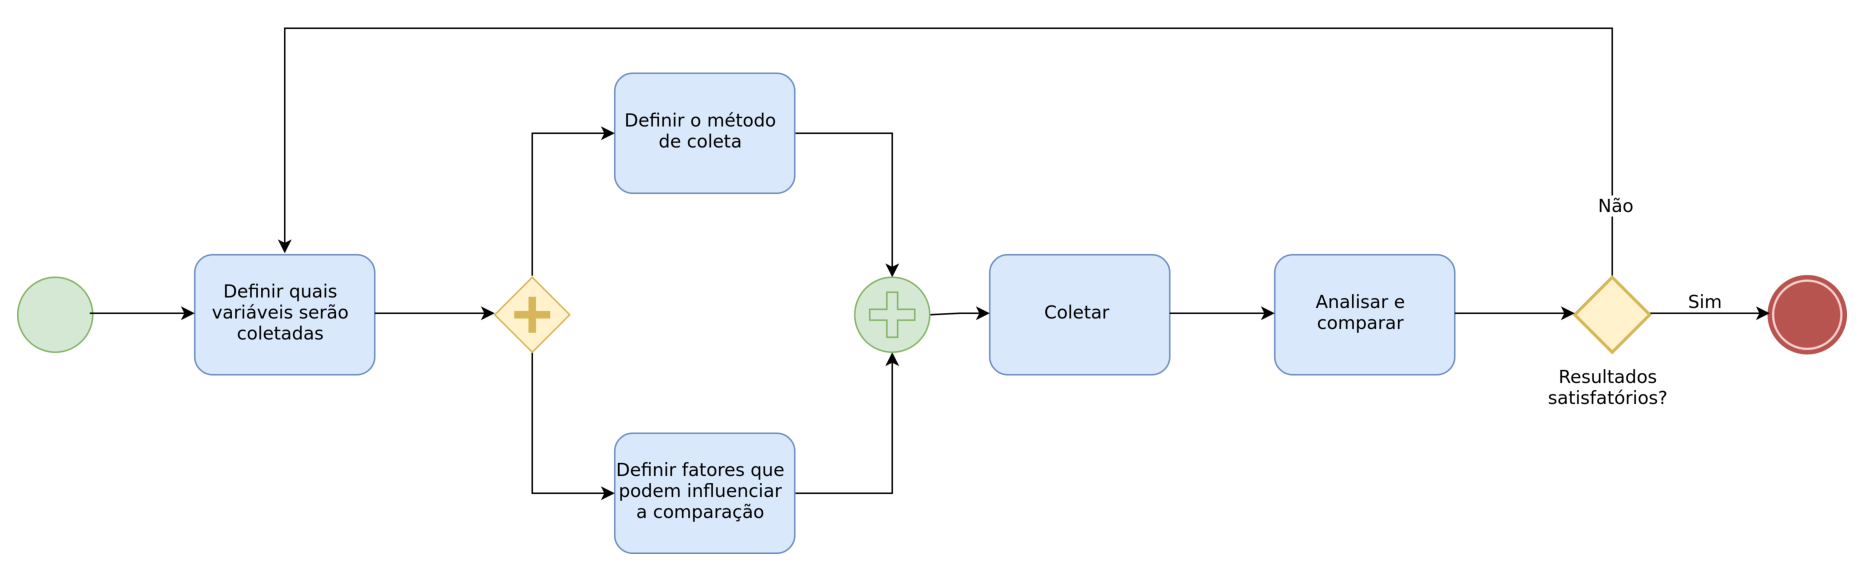
\includegraphics[keepaspectratio=true,scale=0.5]{figuras/metodologiaAnalise.eps}
    \end{figure}

\subsubsection{Etapa 3: Análise comparativa}

Uma vez coletado os dados da etapa anterior, pretende-se fazer uma análise comparativa
entre as fases definidas como objeto de estudo, visando alinhar as diferenças de
escalabilidade e de desenvolvimento referentes a cada uma.

\subsubsection{Etapa 4: Definição das diretrizes}

Com base na análise comparativa realizada e em uma pesquisa exploratória acerca de
desenvolvimento de software escalável, pretende-se elaborar diretrizes para alcançar
um desenvolvimento sustentável e escalável dentro da Rua Dois, elencando possíveis
medidas a serem tomadas dentro da empresa para tal.


\section{Metodologia de desenvolvimento}

A metodologia de desenvolvimento que será aplicada para a execução do presente
projeto será o Scrum. Optou-se por essa metodologia por ser um método iterativo
e incremental, o qual se aplica bem ao contexto de coleta e análise que será
desenvolvido. Além disso, os envolvidos já possuem experiência com o método.

Com base na metodologia de pesquisa adotada na \autoref{sec:MetodologiaPesquisa},
elencou-se no \autoref{quad:TiposDeAtividade} os tipos de atividades a serem
realizadas.

\begin{quadro}
    \caption{Tipos de atividades a serem realizadas\label{quad:TiposDeAtividade}}
    \begin{tabular}{ | c | l | }
    \hline
    \textbf{Abreviatura} &
        \textbf{Descrição} \\ \hline
        S & Estudo \\ \hline
        D & Definição dos métodos de coleta \\ \hline
        C & Coleta \\ \hline
        A & Análise \\ \hline
        E & Escrita \\ \hline
        R & Revisão \\ \hline
    \end{tabular}
\end{quadro}

Tais atividades serão aplicadas sobre os tópicos apresentados no \autoref{quad:Topicos},
visando compor o \textit{product backlog} deste projeto que está exposto
no \autoref{quad:ProductBacklog}. Os identificadores apresentados no
\autoref{quad:ProductBacklog} foram formados pela abreviatura do tipo de atividade com
a numeração do respectivo tópico relacionado.

\begin{quadro}
    \caption{Tópicos a serem abordados durante a execução do projeto\label{quad:Topicos}}
    \begin{tabular}{ | c | l | }
    \hline
    \textbf{Numeração} &
        \textbf{Descrição} \\ \hline
        1 & Arquitetura do sistema \\ \hline
        2 & Qualidade do código \\ \hline
        3 & Práticas de desenvolvimento de software \\ \hline
        4 & Nível de conhecimento da equipe \\ \hline
        5 & Tecnologias utilizadas \\ \hline
        6 & Escalabilidade \\ \hline
        7 & Ciclo de vida de uma \textit{startup} \\ \hline
        8 & Análise comparativa \\ \hline
        9 & Definição das diretrizes \\ \hline
    \end{tabular}
\end{quadro}

\begin{quadro}
    \caption{\textit{Product Backlog} do projeto\label{quad:ProductBacklog}}
    \begin{tabular}{ | c | m{12cm} | }
    \hline
        \textbf{Identificador} &
        \textbf{Descrição} \\ \hline
        S1 & Estudo sobre a arquitetura do sistema \\ \hline
        E1 & Escrita sobre a arquitetura do sistema \\ \hline
        D2 & Definição dos métodos de coleta para qualidade do código \\ \hline
        C2 & Coleta das métricas relacionadas a qualidade do código \\ \hline
        A2 & Análise dos resultados coletados sobre qualidade do código \\ \hline
        E2 & Escrita dos resultados sobre a qualidade do código \\ \hline
        D3 & Definição dos métodos de coleta para práticas de desenvolvimento de software \\ \hline
        C3 & Coleta das métricas relacionadas a práticas de desenvolvimento de software \\ \hline
        A3 & Análise dos resultados coletados sobre as práticas de desenvolvimento de software \\ \hline
        E3 & Escrita dos resultados sobre as práticas de desenvolvimento de software \\ \hline
        D4 & Definição dos métodos de coleta para nível de conhecimento da equipe \\ \hline
        C4 & Coleta das métricas relacionadas ao nível de conhecimento da equipe \\ \hline
        A4 & Análise dos resultados coletados sobre o nível de conhecimento da equipe \\ \hline
        E4 & Escrita dos resultados sobre o nível de conhecimento da equipe \\ \hline
        D5 & Definição dos métodos de coleta para tecnologias utilizadas \\ \hline
        C5 & Coleta das métricas relacionadas as tecnologias utilizadas \\ \hline
        A5 & Análise dos resultados coletados sobre as tecnologias utilizadas \\ \hline
        E5 & Escrita dos resultados sobre as tecnologias utilizadas \\ \hline
        D6 & Definição dos métodos de coleta para escalabilidade \\ \hline
        C6 & Coleta das métricas relacionadas a escalabilidade \\ \hline
        A6 & Análise dos resultados coletados sobre a escalabilidade \\ \hline
        E6 & Escrita dos resultados sobre escalabilidade \\ \hline
        D7 & Definição dos métodos de coleta para ciclo de vida da \textit{startup} \\ \hline
        C7 & Coleta das métricas relacionadas ao ciclo de vida da \textit{startup} \\ \hline
        A7 & Análise dos resultados coletados sobre o ciclo de vida da \textit{startup} \\ \hline
        E7 & Escrita dos resultados sobre o ciclo de vida da \textit{startup} \\ \hline
        A8 & Análise comparativa dos resultados obtidos \\ \hline
        E8 & Escrita a respeito da análise comparativa realizada \\ \hline
        A9 & Análise e definição das diretrizes \\ \hline
        E9 & Escrita da análise e definição das diretrizes \\ \hline
        R  & Revisão
    \end{tabular}
\end{quadro}

Serão executadas \textit{sprints} de 1 semana em um total de 16 \textit{sprints},
iniciando no mês de Fevereiro/2020 e indo até Maio/2020. O \textit{backlog} de cada
\textit{sprint} será definido no início de cada iteração com base no \textit{roadmap}
apresentado no \autoref{quad:Roadmap}.

\begin{quadro}
    \caption{\textit{Roadmap}\label{quad:Roadmap}}
    \begin{tabular}{ | c | l | }
    \hline
    \textbf{Sprint} &
        \textbf{Atividades do \textit{Backlog}} \\ \hline
        1 & S1 e D2 \\ \hline
        2 & E1 e C2 \\ \hline
        3 & A2 e D3 \\ \hline
        4 & E2 e C3 \\ \hline
        5 & A3 e D4 \\ \hline
        6 & E3 e C4 \\ \hline
        7 & A4 e D5 \\ \hline
        8 & E4 e C5 \\ \hline
        9 & A5 e D6 \\ \hline
        10 & E5 e C6 \\ \hline
        11 & A6 e D7 \\ \hline
        12 & E6 e C7 \\ \hline
        13 & A7 e A8 \\ \hline
        14 & E7 \\ \hline
        15 & E8 e A9 \\ \hline
        16 & E9 e R \\ \hline
    \end{tabular}
\end{quadro}

\section{Ferramentas}

As ferramentas que pretende-se usar para a execução deste trabalho são:

\begin{description}
    \item[Artillery] conjunto de ferramentas \textit{open source} escritas em Node.js
    para a realização de testes de carga em servidores. Permite simular vários usuários
    e avaliar fatores como a latência na resposta do servidor.
    \item[CloudWatch] serviço de monitoramento da Amazon que fornece dados e
    \textit{insights} para acompanhar as aplicações. Atualmente já é utilizado na
    Rua Dois e possui o registro de \textit{logs} desde o início da \textit{startup}.
    \item[Draw.io] editor gráfico online que permite a construção de processos e
    desenhos relevantes ao conteúdo apresentado.
    \item[Google Forms] ferramenta para aplicação de questionários e enquetes
    e organização dos resultados para análise. Visa-se utilizá-la para coleta
    de informações referentes aos conhecimento do time de desenvolvimento da Rua Dois.
    \item[Google Planilhas] ferramenta para construção de tabelas e gráficos.
    A qual pretende-se usar para realizar análises sobre os dados coletados.
\end{description}

